\subsubsection{Übernahme stilistischer Elemente}

\hypertarget{RefHeadingToc100333750}{}Von den fast 100 Komponisten der
etwa 200 durch Högn aufgeführten und arrangierten Werke stechen allein
schon wegen dem häufigen Vorkommen ihrer Werke drei Komponisten
deutlich heraus: Vinzenz Goller, Peter Griesbacher und Josef Gruber.
Der Notenbestand in der Ruhmannsfeldener Pfarrkirche St. Laurentius
zeigt hier ein typisches Bild, denn die „großen Drei“ gehörten in der
ersten Hälfte des 20. Jahrhunderts zu den beliebtesten und
bedeutendsten Kirchenkomponisten im süddeutschen Raum. Ihr
stilistischer Einfluss auf Högns Werk verstärkte sich auch dadurch,
dass unter den zahlreichen anderen Komponisten sehr unbekannte
Vertreter mit wenig Vorbildcharakter waren, wie etwa die zum
Bekanntenkreis von Högn zu zählenden Komponisten J. Michael Schöpf, Max
Rauscher, Josef Brunner und Franz Xaver Mitterwallner. Dass sich Högn
angesichts der Allgegenwärtigkeit der drei bedeutenden
Kirchenkomponisten in der alltäglichen Ruhmannsfeldener Kirchenmusik
kaum dem Einfluss auf seine eigenen Werke entziehen konnte oder auch
wollte, unterstreicht die Tatsache, dass einige typische Elemente ihres
Personalstils in Högns Werk wieder zuerkennen sind.

Vinzenz Goller wurde am 9.3.1873 in St. Andrä bei Brixen in Südtirol
geboren und starb am 11.9.1953 in St. Michael im Lungau bei
Salzburg. \footnote{http://www.aeiou.at/aeiou.encyclop.g/g550128.htm}
Nach seinem Studium bei Josef Rheinberger und an der Kirchenmusikschule
in Regens-burg \footnote{Kronsteiner, Seite 18 – 19} übernahm er 1903
seine erste Stelle an Mariä Himmelfahrt in Deggendorf, die er bis 1910
inne hatte. \footnote{Inschrift einer Gedenktafel in der
Stadtpfarrkirche Mariä Himmelfahrt, Deggendorf} Sein Ruf als Komponist
begünstigte schließlich seine Berufung an die Kirchenmusik-Abteilung
der Wiener Akademie für Musik in Klosterneuburg. \footnote{Kronsteiner,
Seite 21}

\begin{center}
\begin{minipage}{4.249cm}
\begin{flushleft}
\tablefirsthead{}
\tablehead{}
\tabletail{}
\tablelasttail{}
\begin{supertabular}{m{4.0490003cm}}

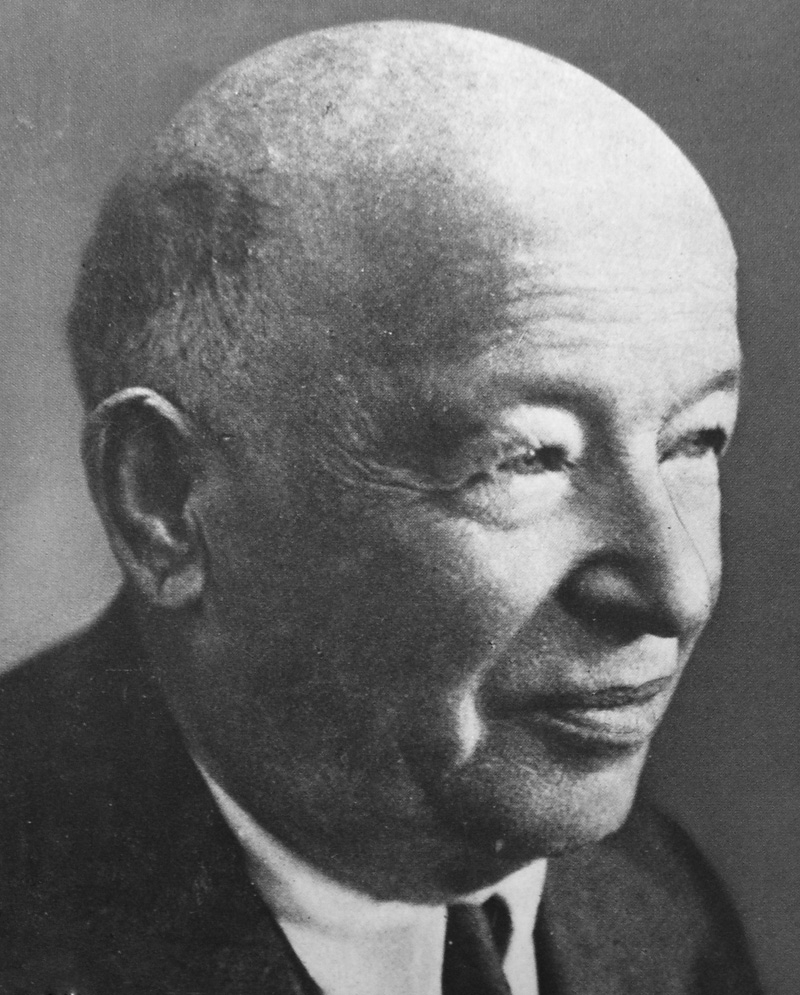
\includegraphics[width=3.866cm,height=4.773cm]{pictures/zulassungsarbeit-img089.jpg}

Abb. \stepcounter{Abb}{\theAbb}: Vinzenz Goller\\
\end{supertabular}
\end{flushleft}
\end{minipage}
\end{center}
Ein gewisser Lokalpatriotismus mag auch dabei gewesen sein, wenn Högn,
ein gebürtiger Deggendorfer, Werke von Goller aufführte, dem ehemaligen
Deggendorfer Kirchenmusiker. Hatte Goller doch in Deggendorf seine
berühmte „Loreto“-Messe geschrieben, die seinen Ruf als hervorragenden
Kirchenkomponist begründete. Es ist daher nicht verwunderlich, dass
Högn nur Werke aufführte, die Goller in seiner Deggendorf Zeit oder
früher geschrieben hatte. \footnote{Kronsteiner, Seite 119 – 121}
Insgesamt waren es 3 Messen, alle 5 Hefte der „Offertorien für das
ganze Kirchenjahr“, 11 Kommunionlieder, 12 Pange
lingua,\textcolor[rgb]{0.6,0.6,0.6}{ }2 Tantum ergo, die
Karfreitags-Kantate, die Fronleichnams-Prozes-sionsgesänge und das
Orgelbuch zum Lob Gottes op. 61, die durch Högn zur Aufführung kamen.

Eine „Spezialität“ in Gollers Kompositionsstil ist der gekonnte Umgang
mit kleinsten Motiven, die er durch Imitation zur größten Entfaltung
bringt. \footnote{Kronsteiner, Seite 30} Diese mit Beethovens
Kompositionsweise zu vergleichende Arbeitstechnik\footnote{
Kronsteiner, Seite 53} ließ sich natürlich gut mit dem traditionellen,
an der altklassischen Vokalpolyphonie orientierenden Stil des strengen
Cäcilianismus verbinden. Unter den neuen Cäcilianern wird deswegen
Goller mit Recht als der Traditionellere bezeichnet. Goller kann Högn
deshalb bei seinen frühen Werken „Pate“ für so manche polyphone Stelle
gestanden haben. Bei den wenigen Imitationen in Högns späten Werken,
lässt sich auch eine Anlehnung an Goller kaum von der Hand weisen.
Ebenso wie Goller versucht Högn hier seine Imitationen mit einer
gemäßigt farbigen, spätromantischen und für Goller typischen Harmonik
zu verbinden.

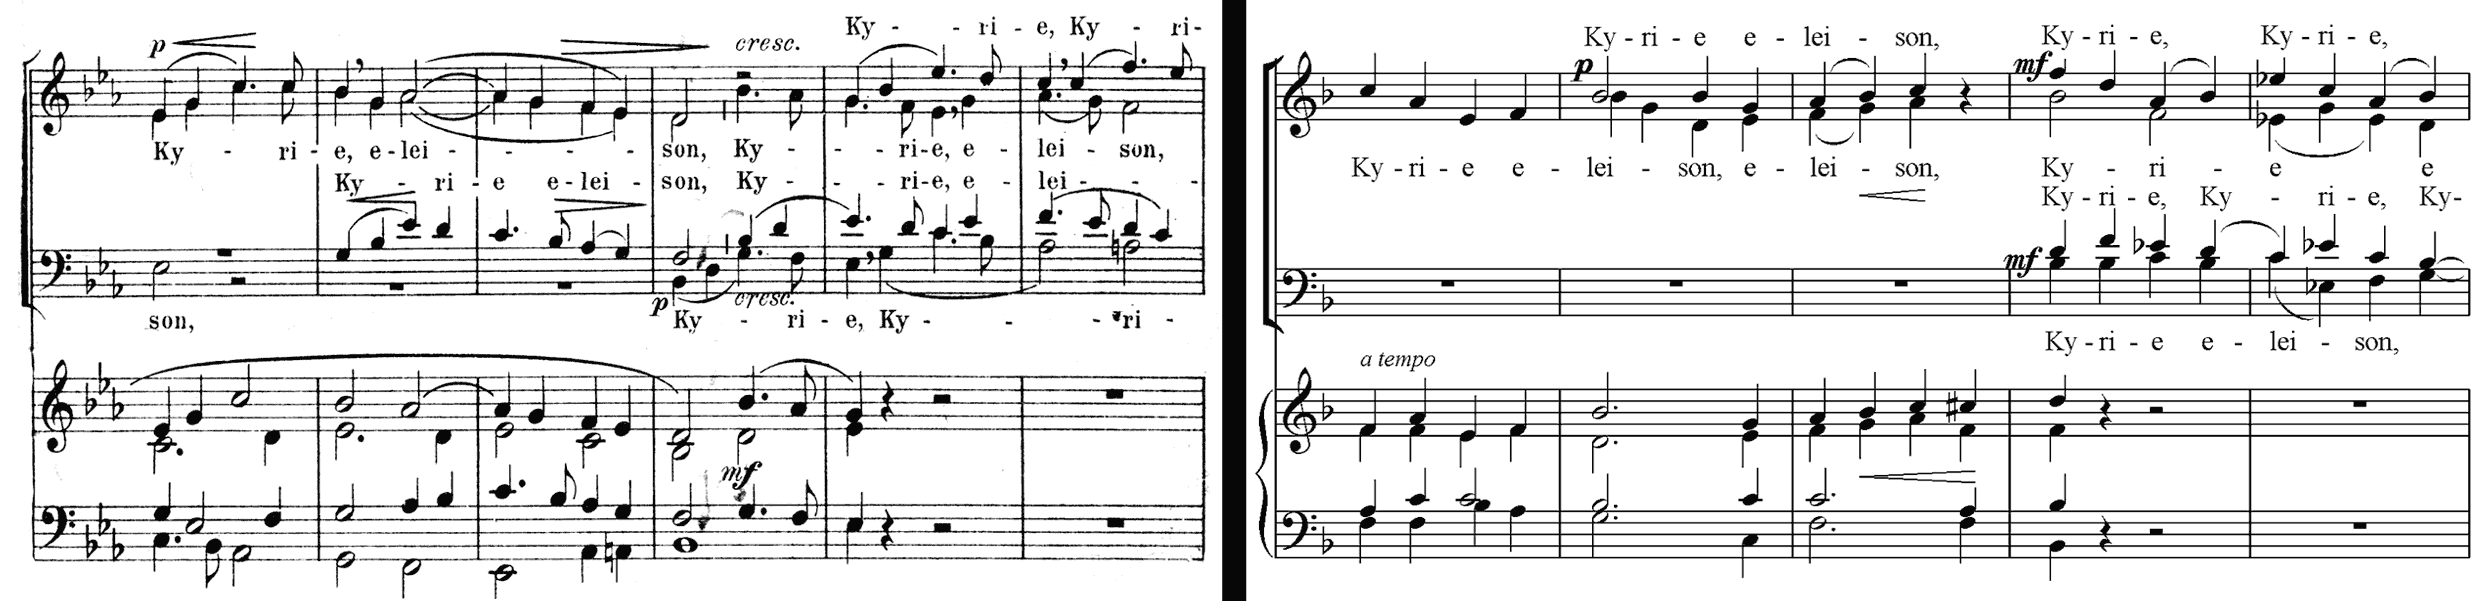
\includegraphics[width=15.977cm,height=3.87cm]{pictures/zulassungsarbeit-img090.png}

Abb. \stepcounter{Abb}{\theAbb}: Goller, „Loreto“-Messe op. 25, Kyrie,
Takt 6 - 11 / Högn, „Josephi“-Messe F-Dur op. 62, Takt 9 - 13

Ein Stück von Högn, das dem Goller-Stil am nächsten kommt, ist das Kyrie
der „Josephi“-Messe. Nicht nur die Bemühungen um ein durch Imitation
aufgelockertes Satzbild und eine liebliche Harmonik, sondern auch die
Verwendung von zwei gegensätzlichen Motiven lassen Assoziationen an
Gollers Kyrie der weltberühmten und von Högn viel verwendeten
„Loreto“-Messe zu.

Peter Griesbacher wurde am 25.3.1864 in Hengersbergmühle bei Egglham
geboren und starb am 28.1.1933 in Regensburg. \footnote{Chrobak, Seite
10} Er erhielt seine erste musikalische Ausbildung in den Passauer
Diözesanseminarien. Ab 1911 war er an der Kirchenmusikschule in
Regensburg als Dozent tätig. Seine kompositorischen Fähigkeiten hatte
sich der Autodidakt durch Studium der alten Meister größtenteils selbst
beigebracht. \footnote{Scharnagl, Griesbacher, Seite 910} An seinen
frühen Werken ist deshalb deutlich der Einfluss der altklassischen
Vokalpolyphonie zu erkennen. Doch schon ab seiner Emmeramsmesse op. 14
ist eine Entwicklung zur einer am Zeitstil orientierten
Kompositionsweise zu erkennen. Besonders auf die Werke Richard Wagners
bezieht sich Griesbacher und dementsprechend sind vermehrt
Stil-Merkmale wie die chromatische Erweiterung des Tonraums, die
orchestrale Behandlung der Orgel und die Leitmotivtechnik, die er zum
ersten Mal in den 1914 entstandenen Ölberggesängen op. 180
einsetzt, \footnote{Chrobak, Seite 24 – 25} in Griesbachers
kirchenmusikalischen Werken zu erkennen. Der zur damaligen Zeit wohl
fortschrittlichste Kirchenkomponist stieß wegen seiner oftmals
\textit{„schrankenloser Chromatik“ } \footnote{Kronsteiner, Seite 31}
auf Widerspruch bei den konservativen Cäcilianern.

\begin{center}
\begin{minipage}{4.076cm}
\begin{flushleft}
\tablefirsthead{}
\tablehead{}
\tabletail{}
\tablelasttail{}
\begin{supertabular}{m{3.8760002cm}}

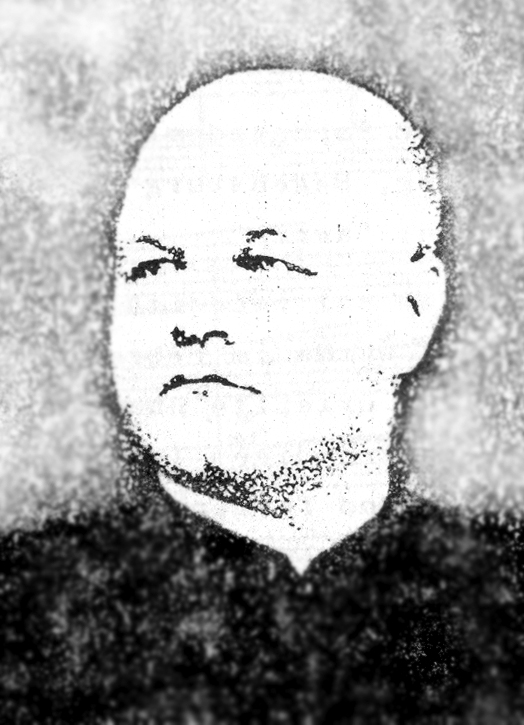
\includegraphics[width=3.694cm,height=5.106cm]{pictures/zulassungsarbeit-img091.jpg}

Abb. \stepcounter{Abb}{\theAbb}: Peter Griesbacher\\
\end{supertabular}
\end{flushleft}
\end{minipage}
\end{center}
August Högn verwendete ausschließlich Werke von Griesbacher, die schon
Elemente des spätromantischem Zeitstils in sich tragen. 4 Messen,
darunter die weltberühmte „Stella-Maris“-Messe Es-Dur op. 141, 11
Marienlieder und die Liedersammlungen Marienpreis \textbf{\textmd{op.
37} }sowie die Lieder zu Ehren des göttlichen Herzens Jesu C-Dur op. 33
beweisen eine rege „Griesbacher“-Rezeption durch Högn.


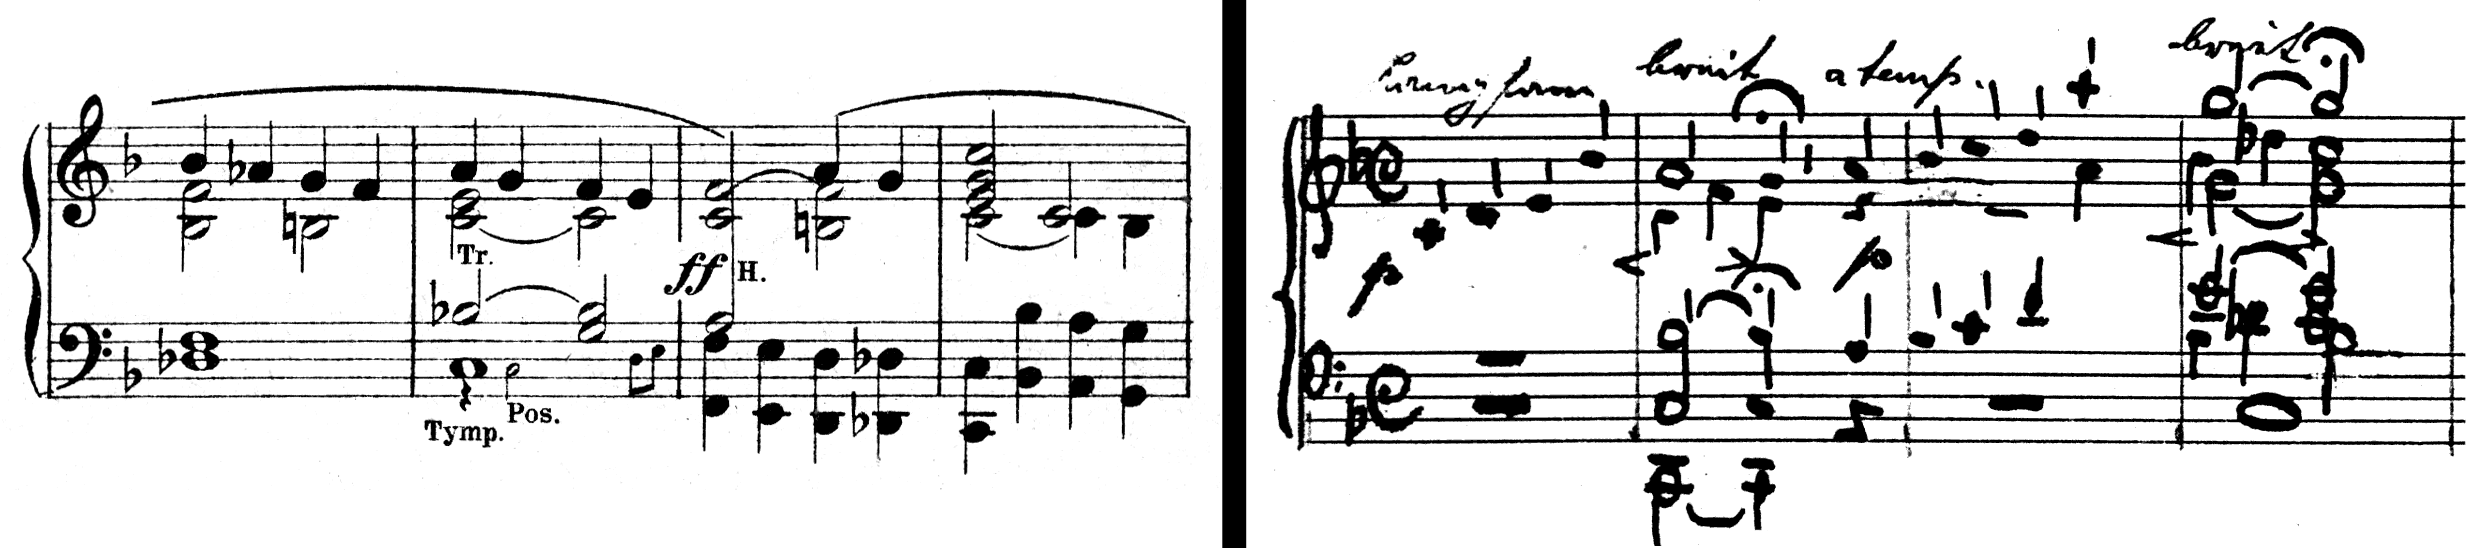
\includegraphics[width=15.977cm,height=3.53cm]{pictures/zulassungsarbeit-img092.png}


Abb. \stepcounter{Abb}{\theAbb}: Griesbacher, Missa in honorem Sti.
Willibaldi op. 123 a, Gloria, Takt 64 – 66 / Högn, „Mater-Dei“-Messe
op. 16, Kyrie, Takt 1 – 4. In beiden Beispielen kommt ein
Dominatseptakkord auf C mit einem a’ als Vorhaltston vor.

An Högns chromatischsten Werken, der „Mater-Dei“-Messe op. 16 und dem
Marienlied Nr. 3 op. 22, sind Einflüsse Griesbachers kaum zu übersehen.
Högn bedient sich bei diesen zwei Werken ähnlich wie Griesbacher
scharfer und ausdrucksstarker chromatischer Harmoniewechsel. Zwar
bilden die harmonischen Schärfen der „Mater-Dei“-Messe und des
Marienlieds Nr. 3 in Högns Werke eher eine Ausnahme, doch auch der
gemäßigte chromatische Tonfall, wie er im Großteil von Högns
musikalischem Schaffen herrscht, könnte durch Griesbacher inspiriert
worden sein.

Der Österreicher Josef Gruber wurde am 18.4.1855 in Wösendorf geboren
und starb am 2.12.1933 in Linz. Unter dem Einfluss von Anton Bruckner,
mehr aber noch durch den Einfluss von Johann Ev. Habert, dessen Schüler
er war, wurde Josef Gruber zu einem typischen Vertreter des
österreichischen Cäcilianismus. \footnote{Quoika, Seite 978} In
Österreich hatte es nie einen vergleichbar strengen cäcilianischen Stil
gegeben, wie er in Deutschland herrschte. \footnote{Seidel, Seite 309}
Das lag unter anderem an Habert, der eine Gegengründung zum Allgemeinen
Cäcilien-Verein initiierte. Stattdessen wurde in Österreich weiterhin
die vom Orchester begleitete Kirchenmusik der Wiener Klassik
gepflegt. \footnote{Kirsch, Seite 321} Die österreichischen
Kirchenkomponisten fanden einen eigenen Stil, der zwischen dem strengen
Cäcilianismus und dem überholten Klassizismus anzusiedeln
war. \footnote{Seidel, Seite 309}

\begin{center}
\begin{minipage}{3.953cm}
\begin{flushleft}
\tablefirsthead{}
\tablehead{}
\tabletail{}
\tablelasttail{}
\begin{supertabular}{m{3.753cm}}

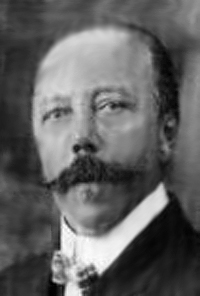
\includegraphics[width=3.57cm,height=5.276cm]{pictures/zulassungsarbeit-img093.jpg}

Abb. \stepcounter{Abb}{\theAbb}: Josef Gruber\\
\end{supertabular}
\end{flushleft}
\end{minipage}
\end{center}
An 5 Messen, 3 Requien, 14 Marienlieder, 4 Tantum ergo und 4 Pangue
lingua von Josef Gruber aus dem Notenbestand der Pfarrkirche St.
Laurentius hat August Högn nachweislich Spuren hinterlassen. Angesichts
dieser langen Liste an Kompositionen besteht wohl kein Zweifel, dass
Grubers Musik eine wichtige Hauptsäule im Kirchemusikrepertoire von
August Högn dargestellt hat.

Die Kompositionen Grubers, die Högn verwendete, waren mit wenigen
Ausnahmen im einfachen homophonen Satz ohne chromatische Erweiterung
geschrieben und weisen deutliche Merkmale einer klassizistischen
Stilistik auf. Diese für Gruber typische Kompositionsweise mag deswegen
richtungweisend für Högns überwiegend homophone Satzweise in seinen
späten Werken gewesen sein. Vom Benedictus der „Josephi“-Messe von Högn
lässt sich nur schwer eine große stilistische Ähnlichkeit mit dem
Benedictus der Missa de Navitate Jesu Christi op. 92 von Gruber
abstreiten. Högn wurde auch schon bei seinen frühen Werken von Gruber
beeinflusst, wie die Orgelbehandlung der „Mater-Dei“-Messe F-Dur op. 16
zeigt. Eine derart ostinate Orgelbegleitung, wie sie Högn im Credo in
den Takten 57 – 62 einsetzt, wäre im strengen cäcilianischen Stil
undenkbar gewesen. Auch die Orgelbegleitung der beiden gemäßigten
Cäcilianer Goller und Griesbacher ist eher figural, an der Linearität
des Chorsatzes orientiert angelegt, als derart akkordisch und
repetitiv.


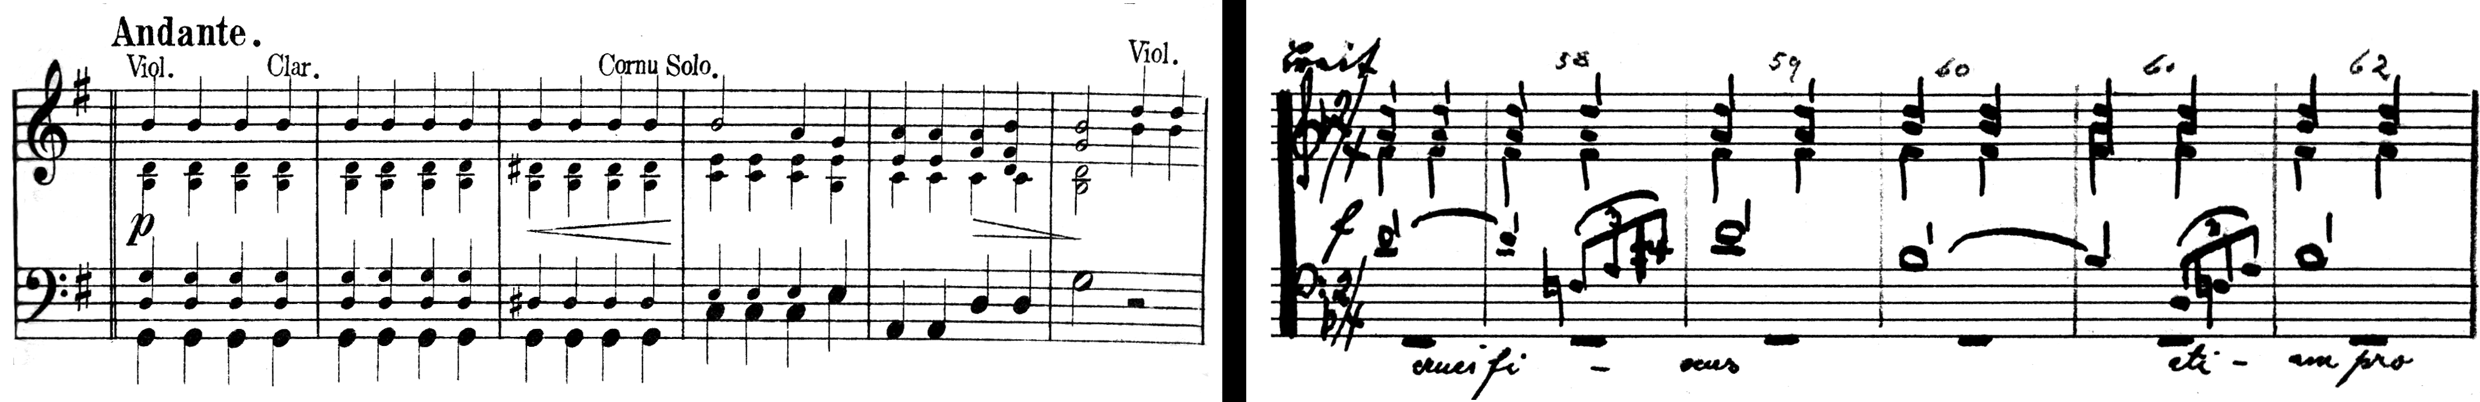
\includegraphics[width=15.977cm,height=2.589cm]{pictures/zulassungsarbeit-img094.png}


Abb. \stepcounter{Abb}{\theAbb}: Gruber, Missa D. N. J. CH op. 92,
Gloria, Qui tollis / Högn, “Mater-Dei“-Messe F-Dur op. 16, Credo, Takt
57 – 62

Wie oben gezeigt wurde, weisen manche Kompositionen von Högn,
beispielsweise die „Mater-Dei“-Messe oder die „Josephi“-Messe mehrere
stilistische Elemente von verschiedenen Komponisten auf. Kann an Högns
Werk aufgrund seiner eklektizistischen Kompositionsweise überhaupt ein
eigener unverwechselbarer Personalstil festgestellt werden? Darauf soll
neben der Frage, welchen stilistischen Veränderungen Högns Werk
unterworfen war, im nächsten Kapitel näher eingegangen werden.